\section{Offline Data Quality Monitoring (Ray)}
\label{sec:monitoring}

Offline data quality monitoring (DQM) provides rapid feedback to the data-taking process.  We expect that offline will be aware of incoming data via the database stream within minutes of the start of a run. Pass1 (see XXX) will run on the data and DQM will run immediately afterwards. We expect DQM will start to appear within a few hours of the start of a run.  Experiment operations will have immediate access.   While the online DQM is the first line of defense, it only has access to very small fraction of some data streams, where the offline DQM will process the full statistics of all data streams.

DQM can be run at any stage. It could be run on raw data before pass1, though it would only have access to raw data and trigger summaries.  DQM will be run on the output of pass1, where can evaluate tracks, calorimeter clusters, and all components of the system. It can be aprt of the calibration process.  It will be run on the final dataset production.

The first component of the system is histogramming.  For simplicity and robustness, we start with histogramming the content of reconstruction output, but anything that can be computed in an art job can be plotted.  The output fo this process is a histogram file, labeled by the process which produced it, the run and subrun involved, and degree of concatenation.  Some quantities will require very little data to be useful, some will require a full run or even many runs.  An arbitrary level of concatenation is allowed.  These histogram files are save to disk r several weeks, then archived to tape.

The second step in the DQM process is to operate on the histogram files and derive metrics.  The metrics might be the mean or RMS of a histogram, the number of hits on a track, or the ratio of matched to unmatched clusters, or normalized quantities, such as the number of CRV hits per time.  These metrics are then labeled as to which histogram file they came from, ans inserted in a database  The DQM database has a standard implementation (see XXXdatabases).  The DQM core system (a nominal set of histograms and metrics) has been running for over a year as part of nightly validation.

The next part of DQM processing is to display the results.  Mu2e supports two display styles. The first is an overlay of histograms.  This might be comparing the current run to the previous, or to a standard set of plots.  We provide several tests of comparison, including a systematic allowance.  The second display style shows the metrics as a timeline.  We allow some selection on the display. The system uses the ploytly package to allow the the user to interact with the plots, for example, dragging to define the time interval.

\begin{figure}[htb]
\begin{center}
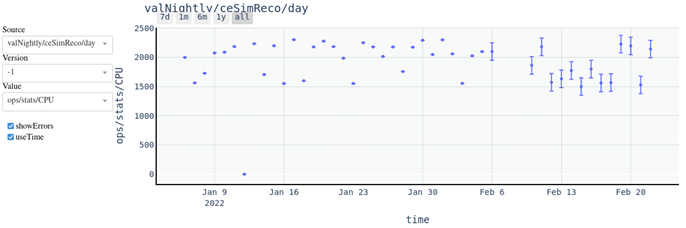
\includegraphics[width=0.9\linewidth]{figures/dqm_timeline.png}
\caption{An example display of a metric timeline}
\label{fig:timeline}
\end{center}
\end{figure}


We provide several standard sets of plots to be viewed by the shift crew and experts.  We will provide tolerances for histogram comparisons or acceptable ranges for the metrics.  If automatic comparisons are out of tolerance, an alarm will be sent to experts.
